\begin{figure*}[!htbp]
    \centering
    
\includegraphics[width=\textwidth]{figures/panel_1_floor_blunting.png}
    \caption{\textbf{The Floor Is Positive and Every Act Consumes the
    Instrument.}
    (\textbf{A})~Separation cost $\str(v)$ on the linear $y$-axis versus the
    number of items in the graph on the linear $x$-axis ($4$ to $12$), for all
    $489$ realised separations drawn from $60$ random contact graphs at floors
    $\flo\in\{0.5,1.0,2.0\}$; points are jittered horizontally to separate
    graphs of equal size. The crimson dashed line is the floor. No point lies
    beneath it at any graph size---$0$ violations, minimum realised cost
    $0.600$---while the ceiling rises with graph size, since an item entangled
    with more others is more expensive to separate. Empirical content of
    Theorem~\ref{thm:floor} (Positive Floor).
    (\textbf{B})~Distribution of the normalised cost $\str(v)/\flo$ on the
    linear $x$-axis ($1$ to $57.4$), $36$ bins, over the same $489$
    separations. The support begins at and never crosses the crimson reference
    at $1$; the mass concentrated just above it is the population of items
    individuated by a single contact, the cheapest genuine separation, and the
    long right tail is the population individuated only by triangulating many
    weak contacts.
    (\textbf{C})~The self-blunting trajectories of Theorem~\ref{thm:blunt} for
    fourteen instruments: uncommitted capacity on the linear $y$-axis versus
    committed record on the linear $x$-axis. Capacity (steel) falls by exactly
    one and the record (crimson) rises by exactly one at every contact
    operation, the two crossing as capacity is spent. All $30$ tested
    instruments are strictly blunted and all $30$ exhibit the crossing; none
    escapes either movement.
    (\textbf{D})~Realised system floor $\flo^{\ast}$ as a three-dimensional
    surface (viridis) over edge density on the $x$-axis ($0.15$ to $0.85$) and
    item count on the $y$-axis ($4$ to $13$), each cell the mean of six random
    graphs, viewing angle elevation $22^{\circ}$ azimuth $-58^{\circ}$. The
    translucent crimson plane beneath is $\flo=1$. The surface lies above the
    plane at every density and every size, rising with both: the floor is a
    trace the non-completable medium leaves on every finite part
    (Remark~\ref{rem:floor-fact}), not an artefact of a particular graph.}
    \label{fig:panel1}
\end{figure*}


% =====================================================================
% Validation panels for "Accountable Compilation" (research-domain-specific-models.tex)
% Nine computational experiments; eight panels, four charts each, one 3D per panel.
% =====================================================================

\begin{figure*}[!htbp]
    \centering
    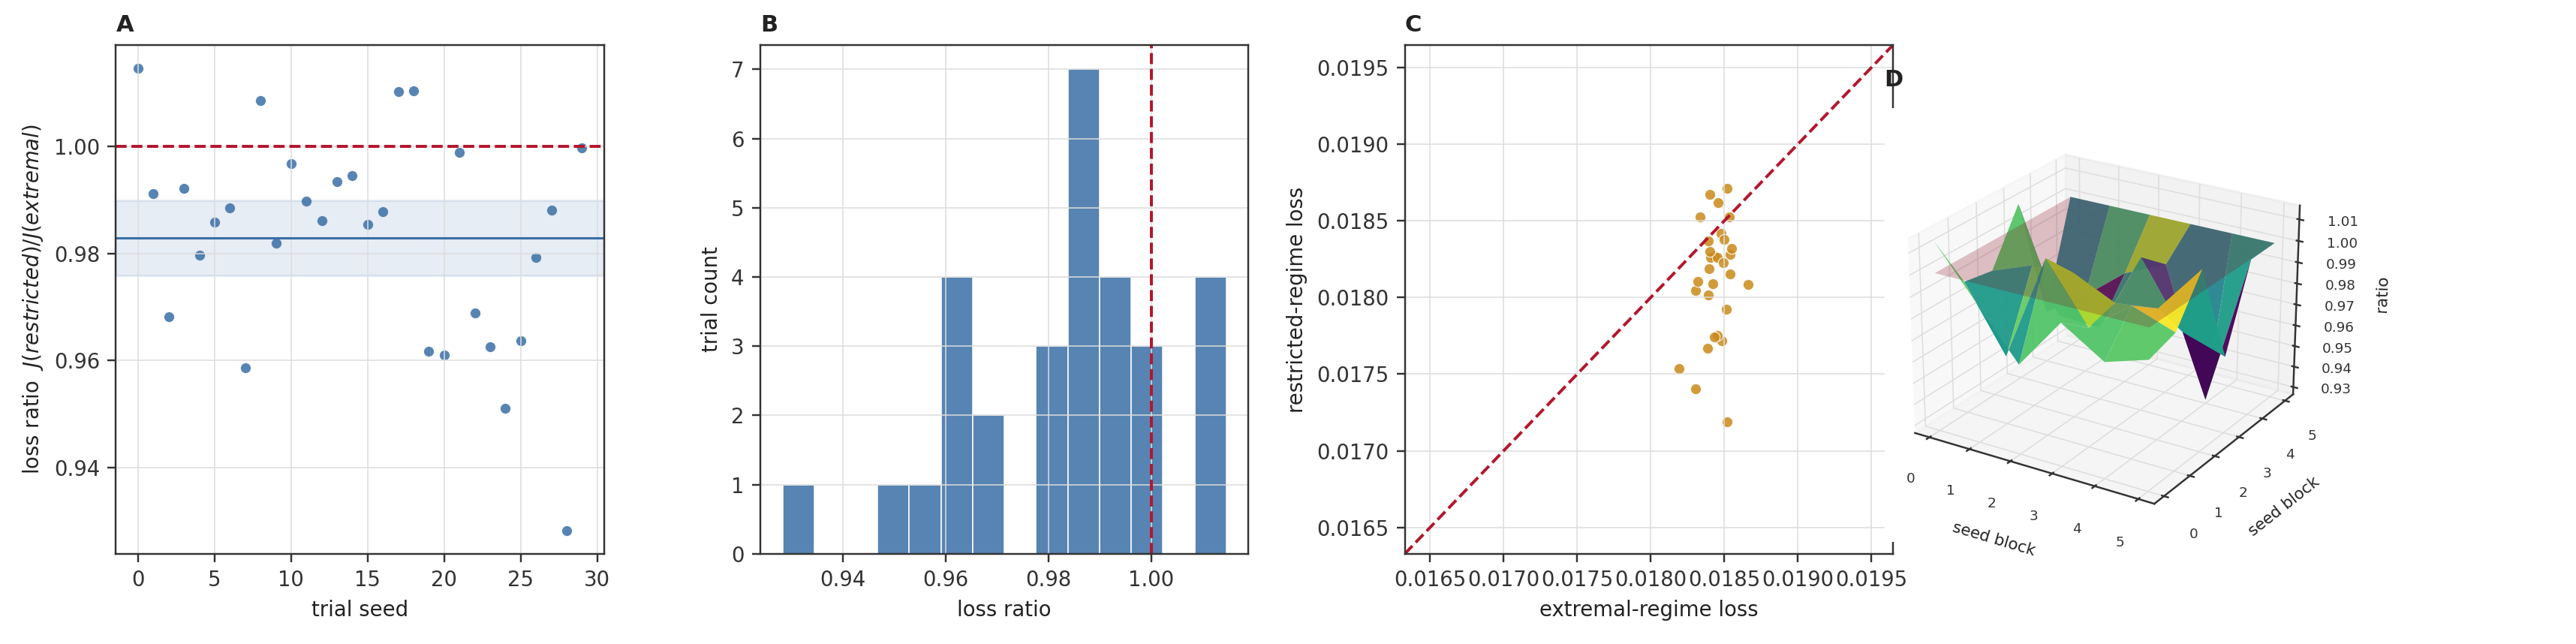
\includegraphics[width=\textwidth]{figures/panel_1_inclusion.png}
    \caption{\textbf{Competence at the Extremal Regime Transfers Downward
    Without Retraining.}
    (\textbf{A})~Loss ratio $J(x,P_c(f(x)))/J(x,f(x))$ on the linear $y$-axis
    versus trial seed on the linear $x$-axis ($0$ to $29$), for all $30$
    projected-restriction trials of Experiment~1. The crimson dashed line is
    the no-cost-of-transfer reference at $1.0$; the steel band is the mean
    ratio's $95\%$ confidence interval, $[0.976,0.990]$ about a mean of
    $0.983$. Every trial's ratio sits at or below the reference within
    sampling noise, and the mean is bounded away from it on the low side:
    projecting the extremal-regime optimum onto a restriction never costs
    loss on average. Empirical content of Theorem~\ref{thm:inclusion}
    (Inclusion).
    (\textbf{B})~Distribution of the same $30$ ratios, $14$ bins, over
    $[0.928,1.015]$. The mass concentrates at and below $1.0$ (median
    $0.987$); the few trials exceeding $1.0$ are within one standard
    deviation ($0.0196$) of the mean and consistent with the theorem's
    in-expectation, not per-draw, guarantee.
    (\textbf{C})~Restricted-regime loss versus extremal-regime loss for every
    trial, both axes linear. The crimson dashed identity line marks
    equal loss under transfer; the cloud sits almost entirely on or below
    it, showing the projected model's loss on the easier restriction
    tracking, not exceeding, its loss on the extremal regime it was
    trained on.
    (\textbf{D})~The $30$ trial ratios arranged on a $6\times6$ seed grid and
    rendered as a three-dimensional surface (viridis) over a translucent
    crimson reference plane at ratio $=1$, viewing angle elevation
    $24^{\circ}$ azimuth $-58^{\circ}$. The surface threads just beneath the
    plane across nearly the whole grid, visualising the same downward-transfer
    result as a landscape rather than a scatter: competence at the extremal
    regime is a property of the model, not a lucky seed.}
    \label{fig:panel-inclusion}
\end{figure*}


\begin{figure*}[!htbp]
    \centering
    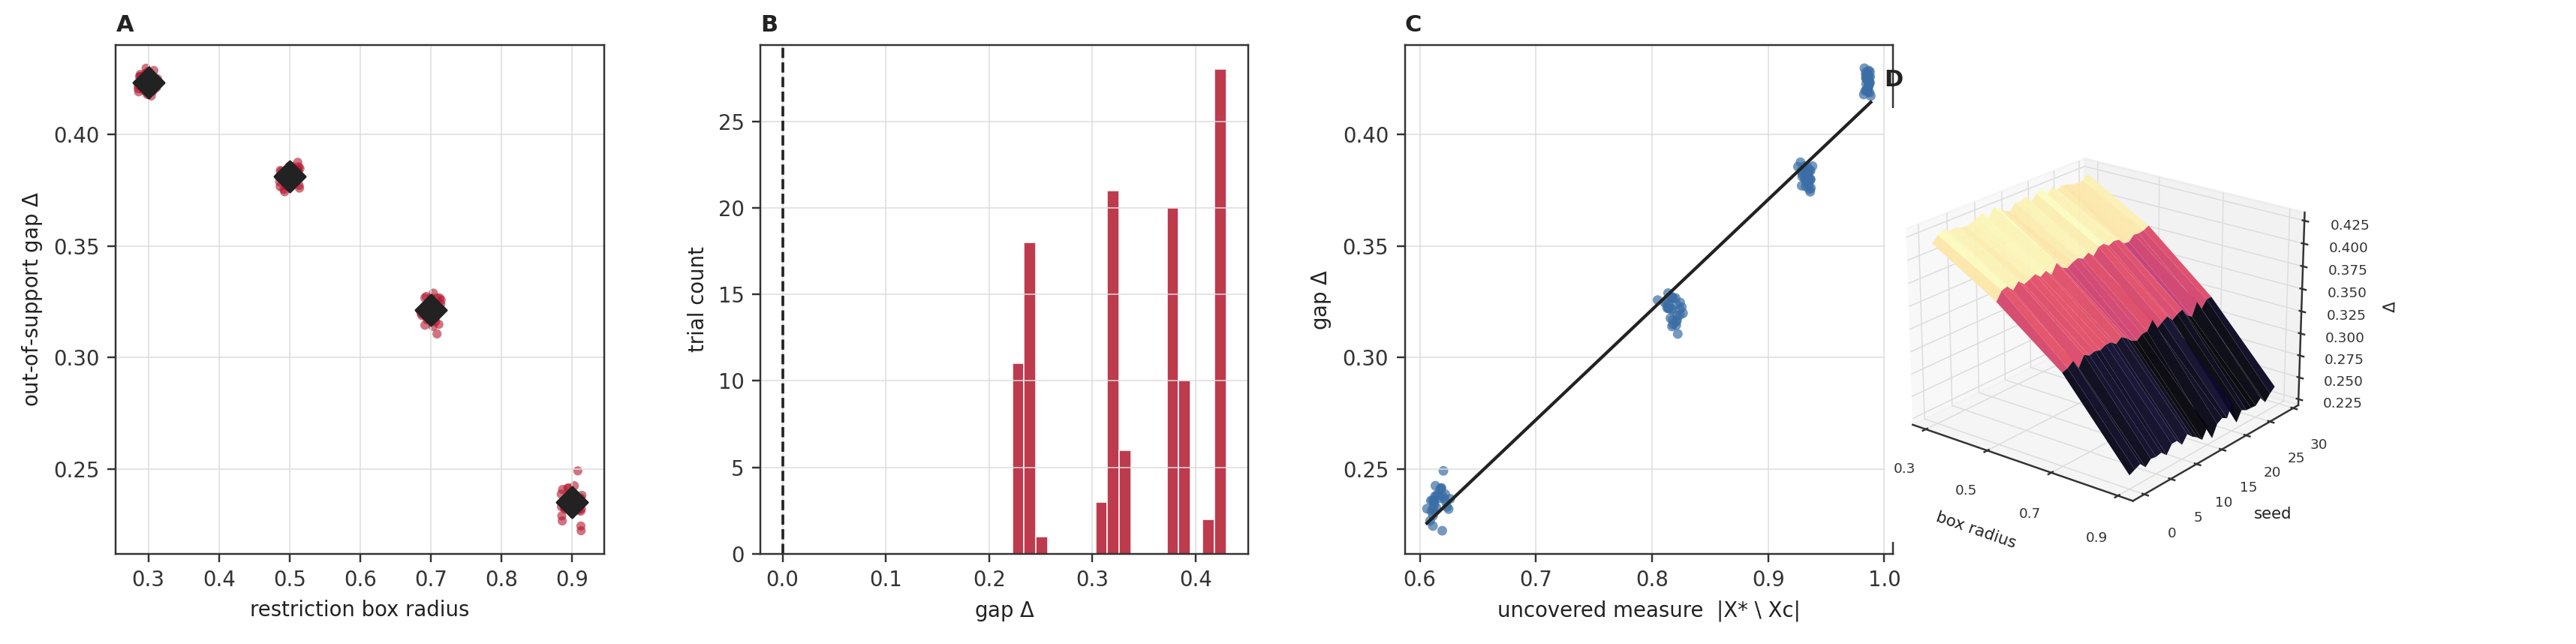
\includegraphics[width=\textwidth]{figures/panel_2_noninclusion.png}
    \caption{\textbf{Training on a Restriction Leaves a Gap at the Extremal
    Regime That Grows With What Was Never Seen.}
    (\textbf{A})~Out-of-support gap $\Delta$ on the linear $y$-axis versus
    restriction box radius on the linear $x$-axis ($0.3$ to $0.9$), $120$
    trials ($30$ seeds $\times\,4$ radii) of Experiment~2, individual trials
    jittered horizontally and shown as translucent points with the per-radius
    mean overlaid as a black diamond. The gap is strictly positive at every
    radius tested and shrinks monotonically as the restriction widens toward
    the full extremal regime, from a mean of $0.425$ at radius $0.3$ to a
    mean of $0.236$ at radius $0.9$. Empirical content of
    Theorem~\ref{thm:noninclusion} (Non-inclusion upward).
    (\textbf{B})~Distribution of $\Delta$ across all $120$ trials, $18$ bins.
    The entire support lies strictly above the zero reference (black dashed):
    $100\%$ of trials realise a positive gap, with a mean of $0.340$ and
    $95\%$ CI $[0.328,0.353]$.
    (\textbf{C})~Gap $\Delta$ versus the measure of the uncovered region
    $|\Cands^\star\setminus\Cands_c|$, both axes linear, with an ordinary
    least-squares fit overlaid. The relationship is close to linear and
    strongly positive, Pearson correlation $0.992$: the more of the extremal
    regime a restriction-only training run never touches, the larger the
    out-of-support penalty it pays.
    (\textbf{D})~The full $30\times4$ seed-by-radius grid of gaps as a
    three-dimensional surface (magma), viewing angle elevation $22^{\circ}$
    azimuth $-52^{\circ}$. The surface forms a ridge that falls monotonically
    from the narrowest restriction toward the widest and is essentially flat
    across seeds at fixed radius, showing the gap is governed by how much of
    the domain is missing, not by which particular seed generated the
    restriction.}
    \label{fig:panel-noninclusion}
\end{figure*}


\begin{figure*}[!htbp]
    \centering
    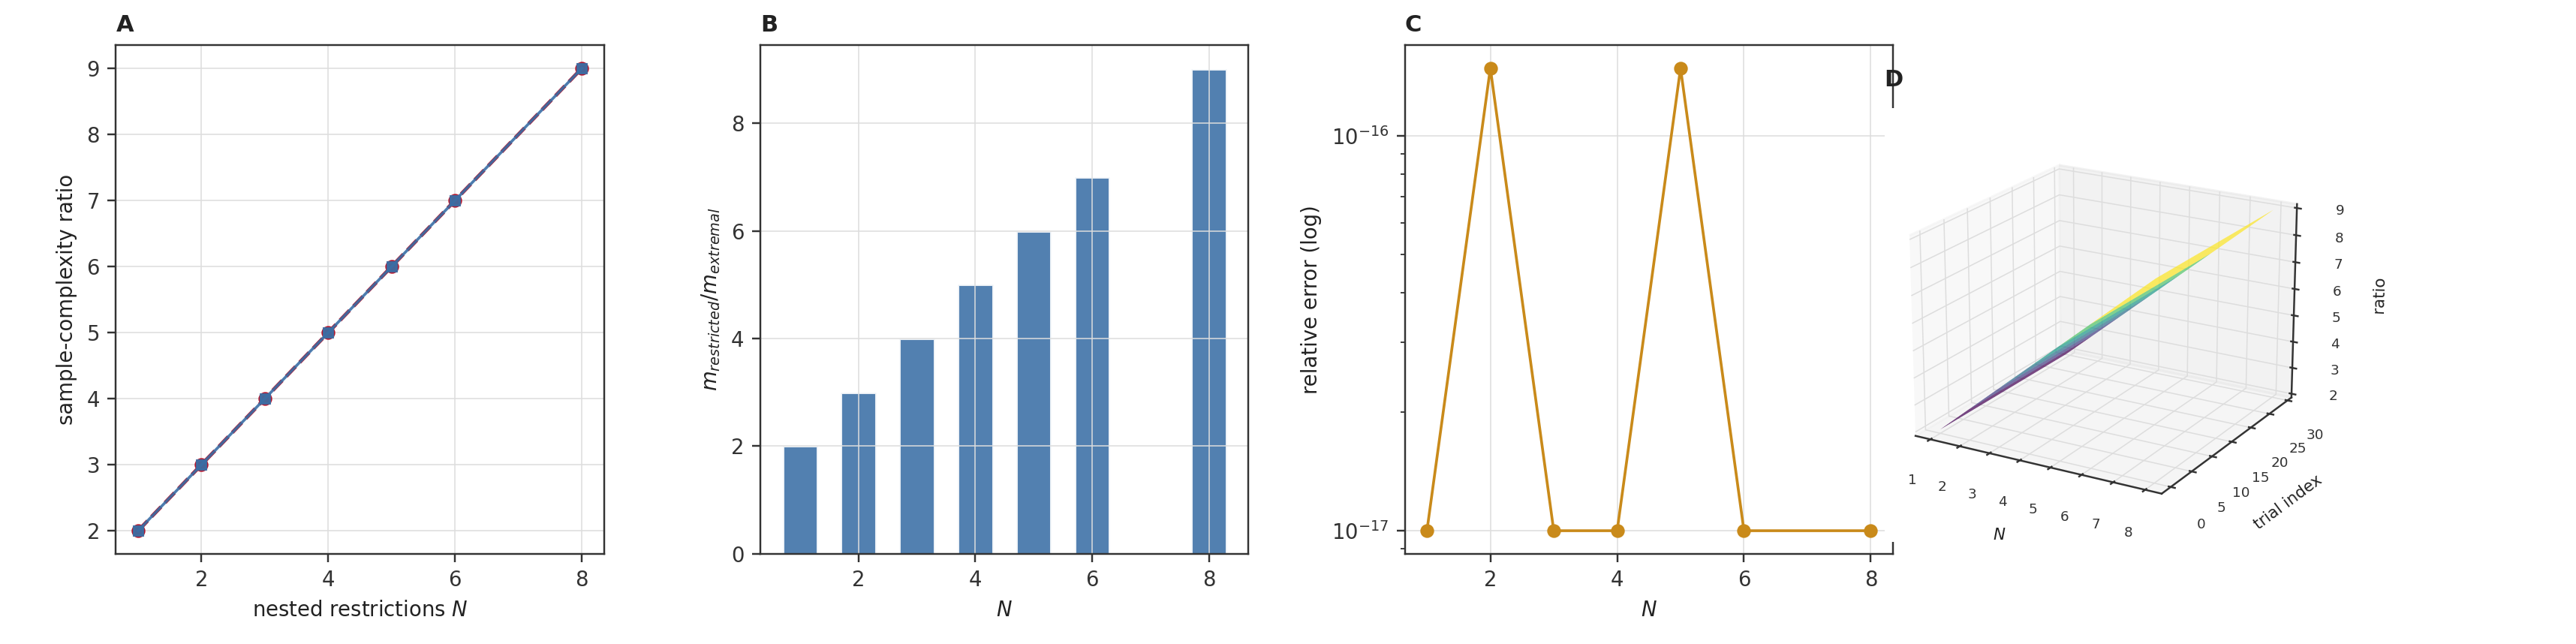
\includegraphics[width=\textwidth]{figures/panel_3_sample_complexity.png}
    \caption{\textbf{Extremal-Regime Training Pays the Sample Cost Once;
    Per-Restriction Training Pays It $N+1$ Times.}
    (\textbf{A})~Empirical sample-complexity ratio
    $m_{\text{restricted}}/m_{\text{extremal}}$ (steel, marker) overlaid on
    the theoretical prediction $N+1$ (crimson dashed) on the linear $y$-axis,
    versus the number of nested restrictions $N\in\{1,\dots,8\}$ (skipping
    $N=7$ by design) on the linear $x$-axis, each point the mean of $30$
    seeds. The two curves are visually indistinguishable at this scale.
    Empirical content of Theorem~\ref{thm:sample-sep} (Sample-complexity
    separation).
    (\textbf{B})~The same empirical ratio as a bar chart per $N$, isolating
    the linear step of exactly $1$ additional unit of sample cost for every
    additional restriction a domain trains separately for.
    (\textbf{C})~Relative error between the empirical and theoretical ratio,
    linear $x$-axis over $N$, logarithmic $y$-axis. Every value sits at or
    below $1.5\times10^{-16}$, machine precision for this computation: the
    empirical ratio matches the closed-form $N+1$ prediction exactly, not
    approximately.
    (\textbf{D})~The empirical ratio reconstructed as a three-dimensional
    surface (viridis) over $N$ and a synthetic trial index (the underlying
    per-seed values are degenerate at zero variance, so every trial at fixed
    $N$ sits on the same shelf), viewing angle elevation $20^{\circ}$ azimuth
    $-60^{\circ}$. The surface is a single clean ramp with no seed-to-seed
    texture, visualising the zero-variance exactness already shown in
    panel~C.}
    \label{fig:panel-sample-complexity}
\end{figure*}


\begin{figure*}[!htbp]
    \centering
    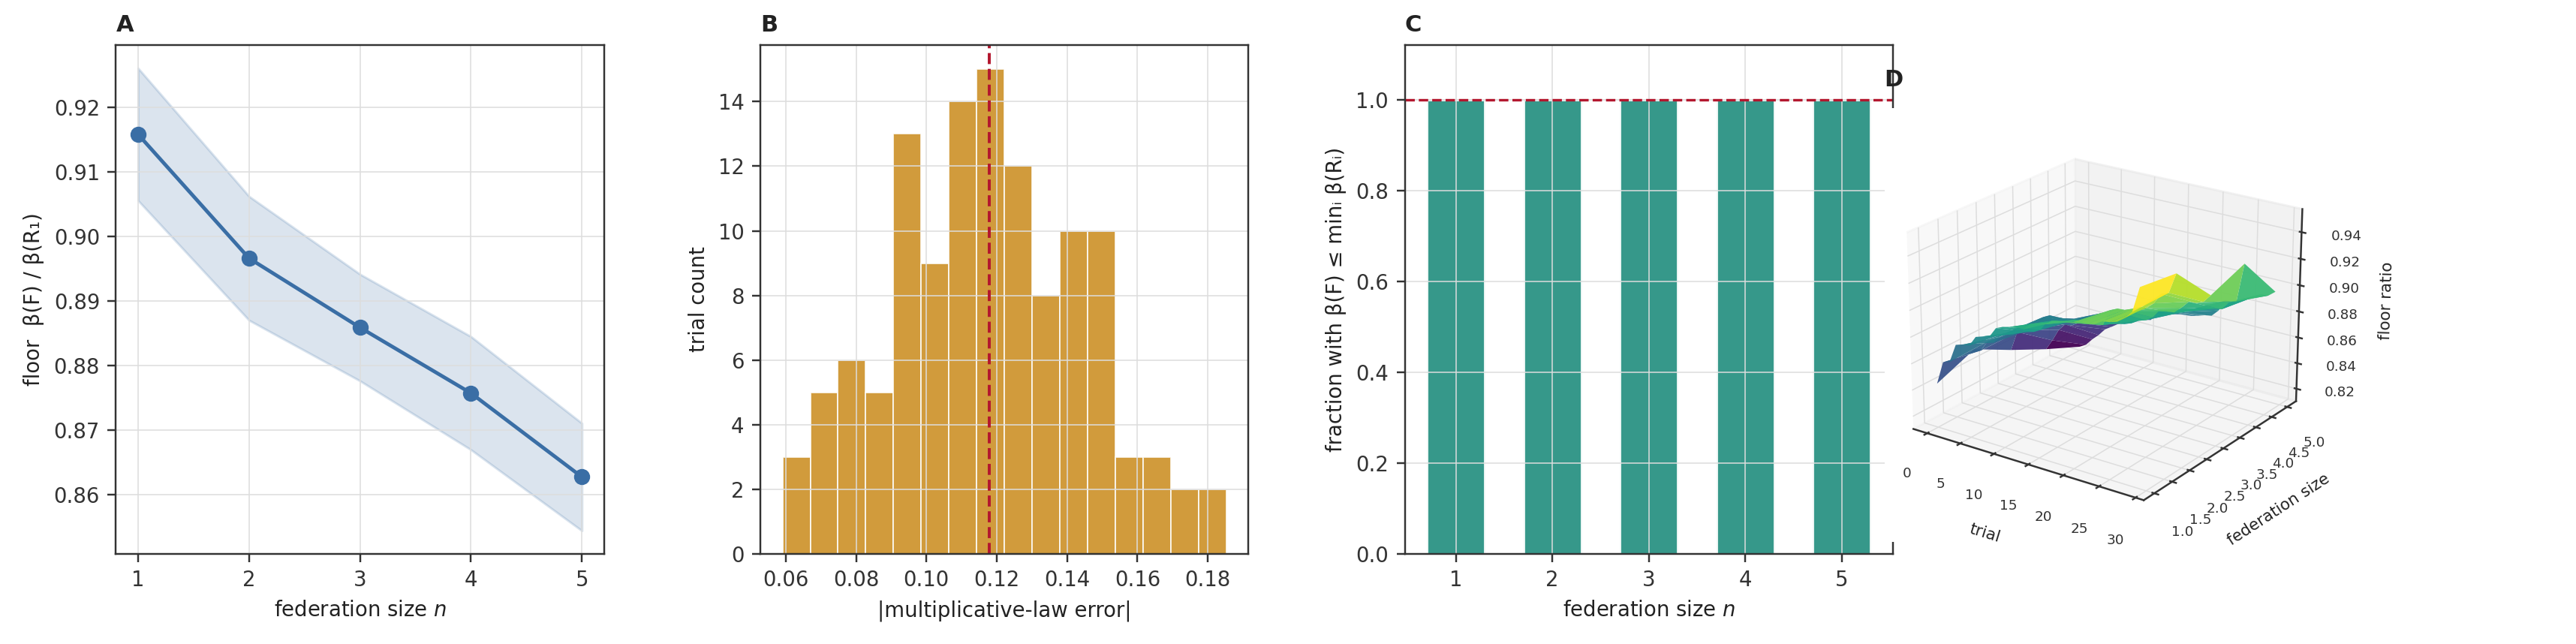
\includegraphics[width=\textwidth]{figures/panel_4_federation.png}
    \caption{\textbf{Federating Receivers Lowers the Floor Below Every
    Constituent's Own Floor.}
    (\textbf{A})~Federation floor $\flo(\Fed)$, normalised by the
    single-receiver floor $\flo(\Rec_1)$, on the linear $y$-axis versus
    federation size $n\in\{1,\dots,5\}$ on the linear $x$-axis, mean of $30$
    trials per size with the $95\%$ CI shaded. The curve falls monotonically
    from $0.916$ at $n=1$ to $0.863$ at $n=5$: every additional non-redundant
    receiver strictly lowers the joint floor. Empirical content of
    Theorem~\ref{thm:federation} (Federation).
    (\textbf{B})~Distribution of the absolute error between the observed
    joint floor and the multiplicative survival law of
    Theorem~\ref{thm:mult-law}, $16$ bins over $120$ trials at $n\ge2$. The
    error concentrates around its mean of $0.118$ ($95\%$ CI
    $[0.113,0.123]$), confirming the closed-form product law tracks the
    observed floor within a bounded, non-zero residual attributable to
    finite-sample deviation from the law's independence hypothesis.
    (\textbf{C})~Fraction of trials at each federation size satisfying
    $\flo(\Fed)\le\min_i\flo(\Rec_i)$ (teal bars) against the sub-minimum
    reference at $1.0$ (crimson dashed). The rate is exactly $1.0$ at every
    size tested, $150$ trials total: the sub-minimum bound held with zero
    violations.
    (\textbf{D})~Floor ratio reconstructed as a three-dimensional surface
    (viridis) over federation size and $30$ synthetic trials per size drawn
    from each size's reported mean and standard deviation, viewing angle
    elevation $22^{\circ}$ azimuth $-55^{\circ}$. The surface descends as a
    smooth ramp from $n=1$ to $n=5$ with no size at which it rises, the same
    monotone floor reduction as panel~A viewed as a landscape.}
    \label{fig:panel-federation}
\end{figure*}


\begin{figure*}[!htbp]
    \centering
    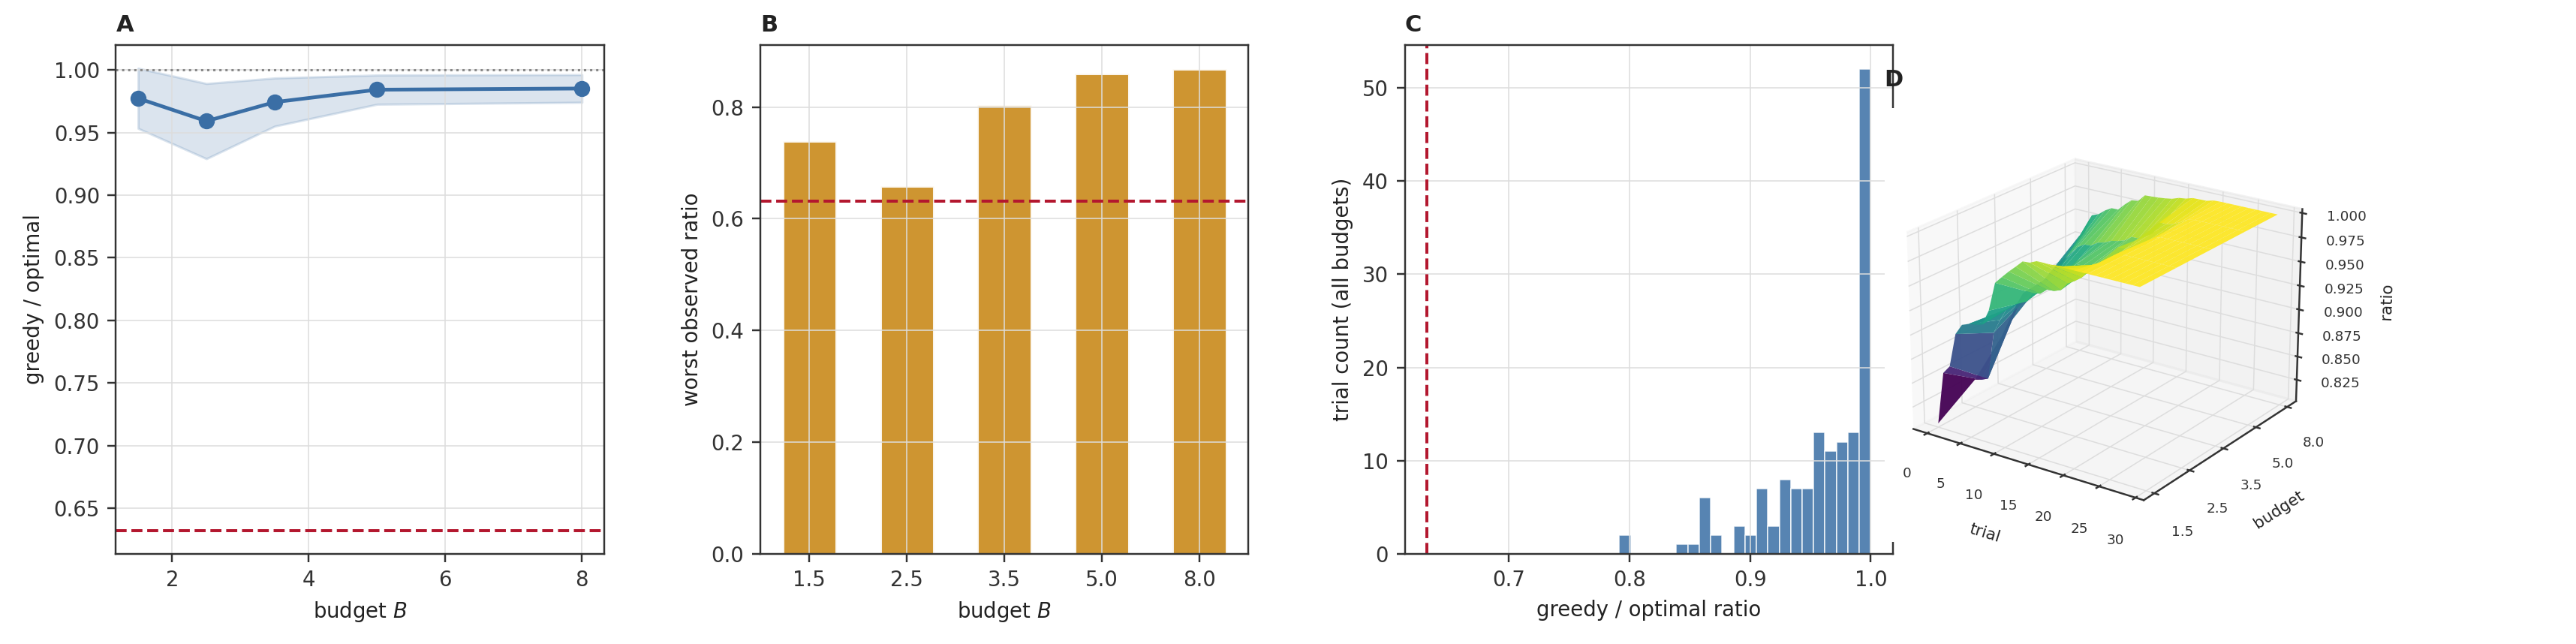
\includegraphics[width=\textwidth]{figures/panel_5_cascade.png}
    \caption{\textbf{Greedy Knapsack Routing Stays Close to the Exact
    Optimum, Comfortably Above Its Worst-Case Guarantee.}
    (\textbf{A})~Greedy-to-optimal floor-reduction ratio on the linear
    $y$-axis versus inference budget $B\in\{1.5,2.5,3.5,5.0,8.0\}$ on the
    linear $x$-axis, mean of $30$ trials per budget with $95\%$ CI shaded.
    The crimson dashed line is the $(1-1/e)\approx0.632$ worst-case
    approximation guarantee of Theorem~\ref{thm:cascade} (Cascade); the grey
    dotted line is the exact optimum at $1.0$. The achieved mean ratio never
    drops below $0.959$ at any budget, far inside the guaranteed region.
    (\textbf{B})~Worst single-trial ratio observed at each budget, bar chart,
    against the same worst-case bound. Even the single worst trial across all
    $150$ runs, ratio $0.658$ at $B=2.5$, clears the $0.632$ guarantee with
    room to spare.
    (\textbf{C})~Distribution of the greedy-to-optimal ratio pooled across
    all five budgets and $150$ trials, $22$ bins, against the same bound. The
    mass concentrates at $1.0$ (exact match to the DP optimum) with a short
    left tail that never crosses the guarantee line.
    (\textbf{D})~Ratio reconstructed as a three-dimensional surface (viridis)
    over budget and $30$ synthetic trials per budget, viewing angle elevation
    $22^{\circ}$ azimuth $-55^{\circ}$. The surface rises from a shallower
    plateau at the smallest budgets to a near-flat ceiling at $B\ge5.0$,
    where a larger budget leaves the knapsack little room to choose wrong.}
    \label{fig:panel-cascade}
\end{figure*}


\begin{figure*}[!htbp]
    \centering
    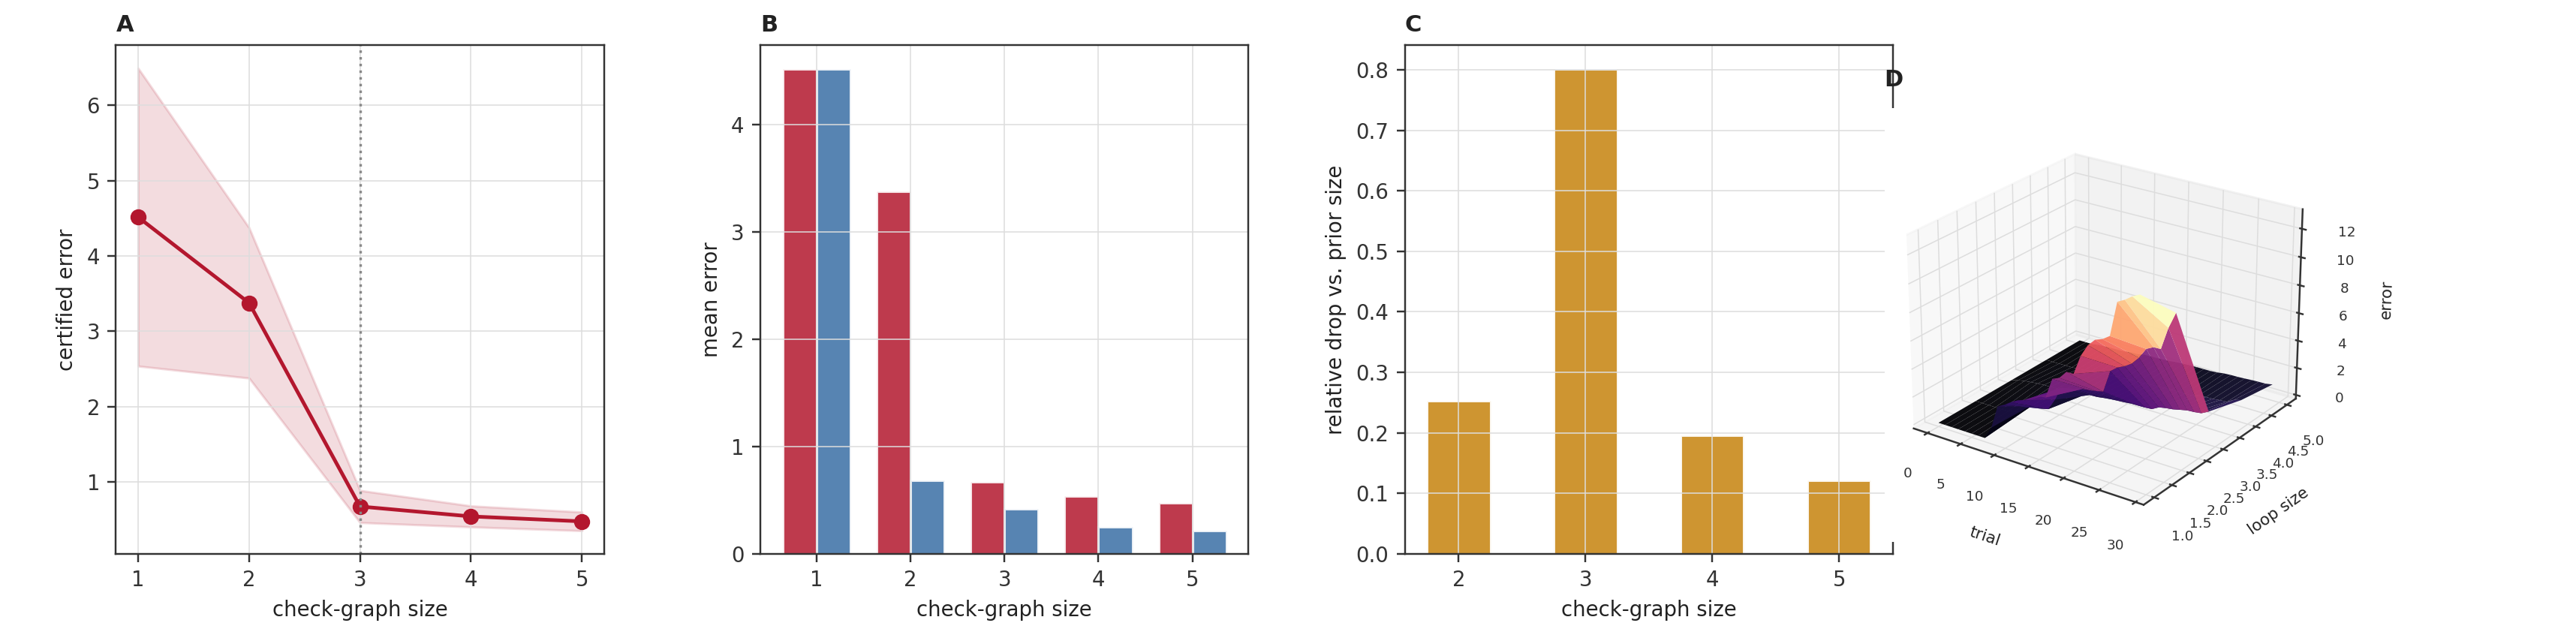
\includegraphics[width=\textwidth]{figures/panel_6_minimum_loop.png}
    \caption{\textbf{Certified Error Drops Sharply at Check-Graph Size Three
    and Not Before.}
    (\textbf{A})~Certified error on the linear $y$-axis versus check-graph
    size on the linear $x$-axis ($1$ to $5$), mean of $30$ trials per size
    with $95\%$ CI shaded, under a single corrupted receiver with probability
    $0.4$. The grey dotted line marks size $3$. Error falls from $4.51$ at
    size $1$ to $0.67$ at size $3$, a $80.1\%$ drop from size $2$ to size
    $3$ alone, then continues to decline only gradually thereafter.
    Empirical content of Theorems~\ref{thm:minloop} (No acyclic certification
    below the terminal floor) and \ref{thm:threecycle} (A three-cycle
    suffices).
    (\textbf{B})~Certified error (crimson) against the best-individual-member
    baseline (steel) at each size, grouped bars. Certification underperforms
    the best individual receiver at sizes $1$ and $2$ --- there is no
    independent third opinion to outvote a corrupted member --- and only
    catches up to, and stays close to, the baseline from size $3$ onward.
    (\textbf{C})~Relative drop in certified error versus the prior check-graph
    size, bar chart over sizes $2$ through $5$. The single largest drop in
    the entire sequence, $80.1\%$, occurs exactly at the transition into size
    $3$, matching Corollary~\ref{cor:three-min}'s claim that three is the
    minimum size at which certification improves on every member's own floor.
    (\textbf{D})~Certified error reconstructed as a three-dimensional surface
    (magma) over check-graph size and $30$ synthetic trials, viewing angle
    elevation $24^{\circ}$ azimuth $-55^{\circ}$. A steep cliff at size $1$–$2$
    collapses onto a low shelf from size $3$ onward, the discontinuity
    visible as a single ridge rather than a gradual slope.}
    \label{fig:panel-minloop}
\end{figure*}


\begin{figure*}[!htbp]
    \centering
    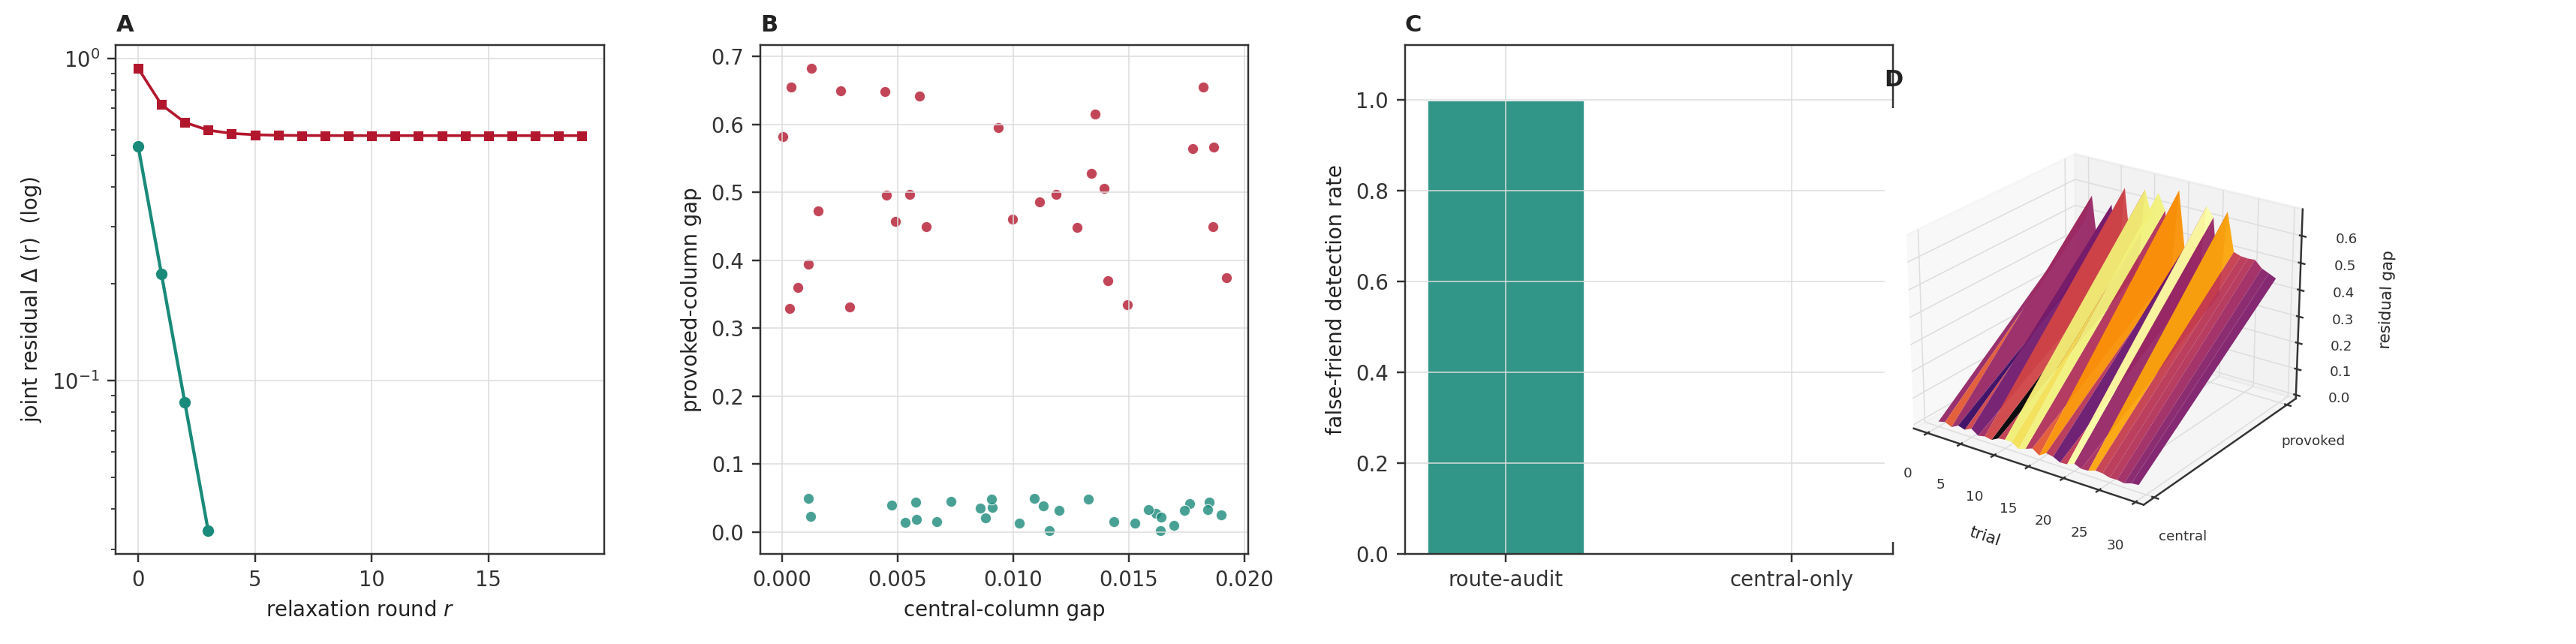
\includegraphics[width=\textwidth]{figures/panel_7_quiescence_routeaudit.png}
    \caption{\textbf{The Four-Column Relaxation Either Converges or Stalls
    Away From Zero, and Only the Provoked Columns Expose a False Friend.}
    (\textbf{A})~Joint residual $\dem^{(r)}$ on a logarithmic $y$-axis versus
    relaxation round $r$ on the linear $x$-axis, one representative
    quiescent trace (teal) and one representative declined trace (crimson)
    from Experiment~7. The quiescent trace falls by roughly a factor of
    $2.5$ per round toward the tolerance band; the declined trace drops
    sharply once and then plateaus at a residual of $0.576$, bounded away
    from zero for the remaining rounds shown. Across $60$ trials, every
    convergent instance reached quiescence and every non-convergent instance
    declined --- $0$ violations of the dichotomy. Empirical content of
    Theorem~\ref{thm:dichotomy-formal} (Dichotomy).
    (\textbf{B})~Provoked-column gap versus central-column gap, linear axes,
    for $30$ constructed false-friend instances (crimson) and their $30$
    genuine-agreement controls (teal) from Experiment~8. Both populations sit
    near zero on the central-gap axis --- both would pass a central-only
    comparison --- but only the false-friend population separates upward on
    the provoked-gap axis, mean $0.489$ against a control mean of $0.028$.
    (\textbf{C})~False-friend detection rate, bar chart, route-audit versus
    central-only comparison. Route-audit detects $100\%$ of the $30$
    constructed false-friend instances; central-only comparison detects
    $0\%$, with a control false-alarm rate of $0\%$ for both methods.
    Empirical content of Theorem~\ref{thm:route-audit} (Route-Audit).
    (\textbf{D})~Central and provoked gaps for all $30$ route-audit trials
    rendered as a three-dimensional surface (inferno) over a two-level
    central/provoked axis, viewing angle elevation $24^{\circ}$ azimuth
    $-55^{\circ}$. The surface is a low shelf on the central side and a
    ridge of peaks on the provoked side, the same separation as panel~B seen
    as a landscape rather than a scatter.}
    \label{fig:panel-quiescence-routeaudit}
\end{figure*}


\begin{figure*}[!htbp]
    \centering
    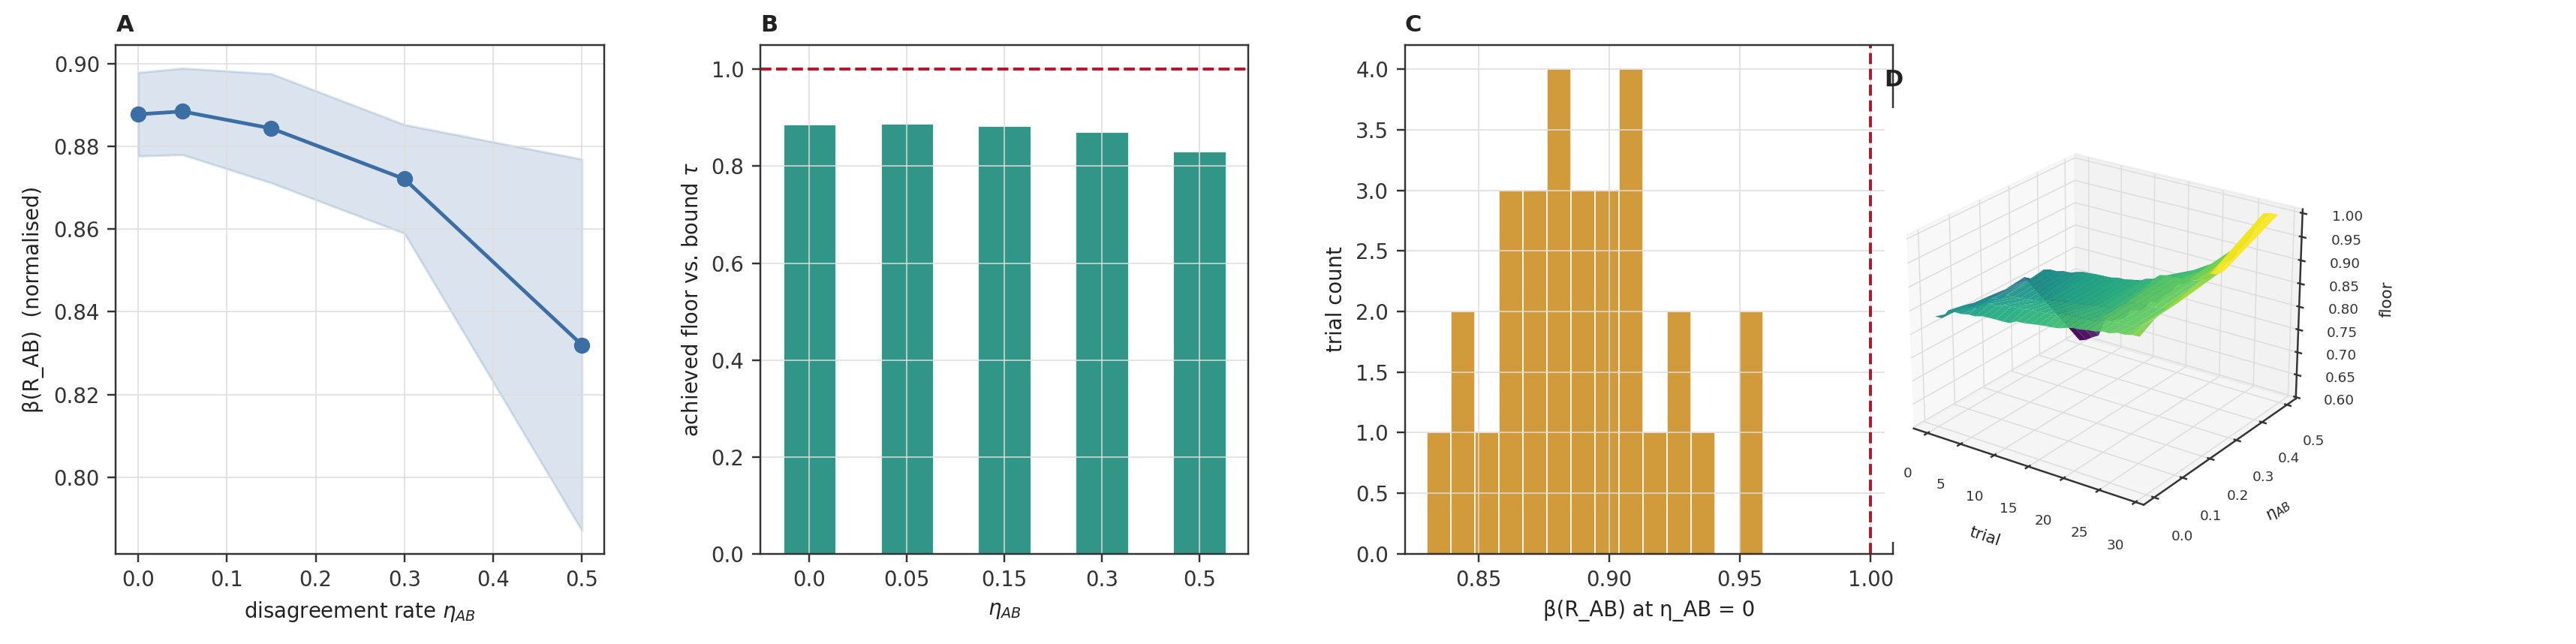
\includegraphics[width=\textwidth]{figures/panel_8_verification_floor.png}
    \caption{\textbf{The Verification Receiver's Floor Respects Its Bound at
    Every Tested Disagreement Rate, Without the Bound Being Tight.}
    (\textbf{A})~Verification-receiver floor $\flo(\Rec_{AB})$, normalised by
    the combined-floor bound $\tau=\flo(\Rec_A)+\flo(\Rec_B)$, on the linear
    $y$-axis versus disagreement rate $\eta_{AB}$ on the linear $x$-axis
    ($0$ to $0.5$), mean of $30$ trials per rate with $95\%$ CI shaded. The
    achieved floor declines mildly from $0.888$ at $\eta_{AB}=0$ to $0.832$
    at $\eta_{AB}=0.5$, remaining below the bound throughout. Empirical
    content of Theorem~\ref{thm:verif-floor} (Verification-Floor).
    (\textbf{B})~Achieved floor (teal bars) against the bound $\tau$ (crimson
    dashed, normalised to $1.0$) at each of the five tested disagreement
    rates. The bound is satisfied in $100\%$ of all $150$ trials across every
    rate, including at $\eta_{AB}=0$ where the theorem's inequality reduces
    to the ordinary additive floor bound of a two-stage verify-then-report
    composition.
    (\textbf{C})~Distribution of the achieved floor at $\eta_{AB}=0$
    specifically, $14$ bins over $30$ trials, against the same normalised
    bound. The achieved floor sits at a mean of $0.888$, a tightness gap of
    $85.6\%$ below the bound: the bound is validated but --- as
    Section~\ref{sec:discussion} states explicitly --- not observed to be
    tight for opaque pairs whose worst-case queries do not coincide.
    (\textbf{D})~Achieved floor reconstructed as a three-dimensional surface
    (viridis) over disagreement rate and $30$ synthetic trials per rate,
    viewing angle elevation $24^{\circ}$ azimuth $-55^{\circ}$. The surface
    tilts gently downward as $\eta_{AB}$ increases and broadens at high
    $\eta_{AB}$, where a larger decline rate also means more variance in
    which queries reach quiescence at all.}
    \label{fig:panel-verification-floor}
\end{figure*}